\documentclass[a4paper,12pt]{extarticle}
\usepackage{geometry}
\usepackage[T1]{fontenc}
\usepackage[utf8]{inputenc}
\usepackage[english,russian]{babel}
\usepackage{amsmath}
\usepackage{amsthm}
\usepackage{amssymb}
\usepackage{fancyhdr}
\usepackage{setspace}
\usepackage{graphicx}
\usepackage{colortbl}
\usepackage{tikz}
\usepackage{pgf}
\usepackage{subcaption}
\usepackage{listings}
\usepackage{indentfirst}
\usepackage[
backend=biber,
style=numeric,
maxbibnames=99
]{biblatex}
\addbibresource{refs.bib}
\usepackage[colorlinks,citecolor=blue,linkcolor=blue,bookmarks=false,hypertexnames=true, urlcolor=blue]{hyperref} 
\usepackage{indentfirst}
\usepackage{mathtools}
\usepackage{booktabs}
\usepackage[flushleft]{threeparttable}
\usepackage{tablefootnote}

\usepackage{chngcntr} % нумерация графиков и таблиц по секциям
\counterwithin{table}{section}
\counterwithin{figure}{section}

\graphicspath{{graphics/}}%путь к рисункам

\makeatletter
% \renewcommand{\@biblabel}[1]{#1.} % Заменяем библиографию с квадратных скобок на точку:
\makeatother

% \geometry{left=2.5cm}% левое поле
% \geometry{right=1.0cm}% правое поле
\geometry{left=1.75cm}
\geometry{right=1.75cm}

\geometry{top=2.0cm}% верхнее поле
\geometry{bottom=2.0cm}% нижнее поле
\setlength{\parindent}{1.25cm}
\renewcommand{\baselinestretch}{1.5} % междустрочный интервал


\newcommand{\bibref}[3]{\hyperlink{#1}{#2 (#3)}} % biblabel, authors, year
\addto\captionsrussian{\def\refname{Список литературы (или источников)}} 

\renewcommand{\theenumi}{\arabic{enumi}}% Меняем везде перечисления на цифра.цифра
\renewcommand{\labelenumi}{\arabic{enumi}}% Меняем везде перечисления на цифра.цифра
\renewcommand{\theenumii}{.\arabic{enumii}}% Меняем везде перечисления на цифра.цифра
\renewcommand{\labelenumii}{\arabic{enumi}.\arabic{enumii}.}% Меняем везде перечисления на цифра.цифра
\renewcommand{\theenumiii}{.\arabic{enumiii}}% Меняем везде перечисления на цифра.цифра
\renewcommand{\labelenumiii}{\arabic{enumi}.\arabic{enumii}.\arabic{enumiii}.}% Меняем везде перечисления на цифра.цифра

% Мои пакеты
\usepackage{tabularx}
\usepackage{booktabs}
\usepackage{pifont}

\newcommand{\cmark}{\ding{51}}
\newcommand{\xmark}{\ding{55}}
\usepackage{xcolor}

\begin{document}
\begin{titlepage}
\newpage

{\setstretch{1.0}
\begin{center}
ПРАВИТЕЛЬСТВО РОССИЙСКОЙ ФЕДЕРАЦИИ\\
ФГАОУ ВО НАЦИОНАЛЬНЫЙ ИССЛЕДОВАТЕЛЬСКИЙ УНИВЕРСИТЕТ\\
«ВЫСШАЯ ШКОЛА ЭКОНОМИКИ»
\\
\bigskip
Факультет компьютерных наук\\
Образовательная программа «Прикладная математика и информатика»
\end{center}
}

\vspace{7em}

\begin{center}
{\bf ВЫПУСКНАЯ КВАЛИФИКАЦИОННАЯ РАБОТА}\\
%Выберите какой у вас проект
{\bf Исследовательский проект на тему:}\\
%{\bf Программный проект на тему:}\\
%{\bf Отчет о командном программном проекте на тему:}\\
{\bf Оптимизация размера сенсоров для физики элементарных частиц}\\
\end{center}

\vspace{2em}

{\bf Выполнил студент: \vspace{2mm}}

{\setstretch{1.1}
\begin{tabular}{l@{\hskip 1.5cm}l}
группы \#БПМИ203, 4 курса & Зиманов Алихан
\end{tabular}}

% Обычно у вас есть один научный руководитель, и это человек, с которым вы работаете над проектом. Иногда по формальным причинам у вас будет руководитель (штатный сотрудник Вышки) и соруководитель (тот, с кем вы работаете), — об этом вам сообщит учебный офис (в случае с ВКР) или ЦППРиП (в случае с курсовым проектом). Также, если кто-то дополнительно вам помогал, то его можно указать как консультанта. 

%ваш официальный научник (из ВШЭ)
\vspace{1em}
{\bf Принял руководитель ВКР: \vspace{2mm}}

{\setstretch{1.1}
\begin{tabular}{l}
Болдырев Алексей Сергеевич\\
Научный сотрудник\\
Факультет компьютерных наук НИУ ВШЭ 
\end{tabular}}

% со-руководитель (если есть)
%\vspace{1em}
%{\bf Соруководитель: \vspace{2mm}}%это ваш официальный научник

%{\setstretch{1.1}
%\begin{tabular}{l}
%Петрова Надежда Александровна\\
%Инженер-исследователь\\
%ОАО Компания "Нейросети и деревья" 
%\end{tabular}}

% консультант (если есть)
%\vspace{1em}
%{\bf Консультант: \vspace{2mm}}%это ваш официальный научник

%{\setstretch{1.1}
%\begin{tabular}{l}
%Иванова Надежда Александровна\\
%Инженер-исследователь\\
%ОАО Компания "Нейросети и деревья" 
%\end{tabular}}

\vspace{\fill}

\begin{center}
Москва 2024
\end{center}

\end{titlepage}% это титульный лист - выберите подходящий вам из имеющихся в проекте вариантов (kr - курсовая работа у 3 курса, vkr - выпускная квалификационная работа у 4 курса)
\newpage
\setcounter{page}{2}

{
	\hypersetup{linkcolor=black}
	\tableofcontents
}

\newpage

\newpage

\section*{Аннотация}   % this is how to use russian
Эксперименты по физике частиц часто связаны с точным измерением энергии и положения частиц, таких как фотоны, взаимодействующих с детекторами типа электромагнитных калориметров. Оптимизация размера сенсора этих детекторов имеет решающее значение для получения точных реконструкций свойств частиц с учетом экономической эффективности. В этом исследовании мы изучаем оптимизацию размера датчика для экспериментов по физике частиц, уделяя особое внимание реконструкции энергии фотонов и их положения в калориметре. Мы предлагаем использовать методы глубинного обучения для решения этой задачи и оценить различные разрешения датчиков от $10 \times 10$ до $40 \times 40$ при фиксированном физическом размере калориметра. Наш подход предполагает обучение моделей глубинного обучения, включая архитектуры ResNet18 и Vision Transformer, и сравнение их качества с базовыми моделями, такими как аналитическая модель и линейная регрессия. Мы используем такие метрики, как средняя квадратичная ошибка (MSE), средняя абсолютная ошибка (MAE), корень из средней квадратичной ошибки (RMSE), а также взвешенные версии этих метрик для оценки точности реконструкции для датчиков разного размера. Кроме того, мы изучили влияние функций потерь, стратегий обучения и параметров моделей на качество работы моделей глубинного обучения. Полученные нами результаты подчеркивают важность выбора оптимального разрешения сенсоров, обеспечивающего баланс между точностью реконструкции и экономической эффективностью при проведении экспериментов по физике частиц.

\addcontentsline{toc}{section}{Аннотация}

\section*{Ключевые слова}
Физика элементарных частиц, оптимизация размера сенсоров, глубинное обучение, компьютерное зрение, реконструкция энергии фотонов, БАК, электромагнитные калориметры

\section*{Abstract}   % this is how to use russian
Particle physics experiments often involve the precise measurement of energy and position of particles, such as photons, interacting with detectors like electromagnetic calorimeters. Optimizing the sensor size of these detectors is crucial for achieving accurate reconstructions of particle properties while considering cost-effectiveness. In this research, we explore the optimization of sensor size for particle physics experiments, focusing on the reconstruction of photon energy and position within calorimeter cells. We propose using deep learning methods to address this task and evaluate various sensor granularities ranging from $10 \times 10$ to $40 \times 40$ keeping the same physical size of the calorimeter. Our approach involves training deep learning models, including ResNet18 and Vision Transformer architectures, and comparing their performance against baseline models such as analytical formula-based model and Linear Regression. We employ metrics like Mean Squared Error (MSE), Mean Absolute Error (MAE), Root Mean Squared Error (RMSE), and weighted versions of these metrics to assess the reconstruction accuracy across different sensor granularities. Additionally, we investigate the impact of loss functions, training strategies, and model parameters on the performance of the deep learning models. Our findings highlight the importance of selecting an optimal sensor size that balances reconstruction accuracy and cost-effectiveness for particle physics experiments.

\addcontentsline{toc}{section}{Abstract}

\section*{Keywords}
Particle Physics, Sensor Optimization, Deep Learning, Computer Vision, Photon Energy Reconstruction, LHC, ECAL

\pagebreak

\section{Введение}
\label{section:introduction}

\colorbox{yellow}{Добавить ссылки на всю используемую литературу}

Эксперименты по физике элементарных частиц направлены на раскрытие фундаментальных структурных элементов Вселенной и сил, управляющих их взаимодействием. Эти эксперименты часто связаны со столкновением частиц высоких энергий и последующим измерением и анализом свойств частиц, образующихся при этих столкновениях. В таких экспериментах детекторы играют ключевую роль в улавливании признаков различных частиц, включая фотоны, электроны, мюоны, нейтрино и другие. Среди различных типов детекторов, используемых в экспериментах по физике частиц, электромагнитные калориметры предназначены для измерения энергии частиц, в частности фотонов и электронов, с высокой точностью.

Электромагнитные калориметры обычно состоят из плотных материалов, таких как свинец или вольфрам, расположенных слоями, перемежающимися с чувствительными элементами, обычно изготовленными из таких материалов, как кремний или сцинтилляционные кристаллы. Когда высокоэнергетические фотоны или электроны взаимодействуют с материалами калориметра, они создают электромагнитные ливни, являющиеся каскадом испускания вторичных и последующих частиц. Энергия, накопленная этими частицами в калориметре, измеряется чувствительными элементами, предоставляя ценную информацию об энергии и положении падающих частиц. Пример электромагнитного калориметра и электромагнитного ливня можно увидеть на Рисунке~\ref{image:ecal}.

Одним из важнейших аспектов при разработке и оптимизации электромагнитных калориметров является выбор размера датчика. Под размером датчика понимаются размеры отдельных чувствительных элементов калориметра, которые напрямую влияют на зернистость и пространственное разрешение детектора. Более мелкая детализация, достигаемая за счет использования датчиков меньшего размера, позволяет лучше локализовать осаждение энергии в ячейках калориметра, что приводит к улучшению пространственного разрешения и реконструкции энергии. Однако уменьшение размера датчика сопряжено с определенными трудностями, включая повышение сложности считывания данных с датчика, увеличение стоимости изготовления и потенциальное ухудшение соотношения сигнал/шум.

Оптимизация размера датчика для электромагнитных калориметров предполагает поиск баланса между точностью реконструкции и экономической эффективностью. Хотя датчики меньшего размера обеспечивают более тонкое пространственное разрешение и потенциально более высокую точность реконструкции, они не всегда могут быть практичными или экономичными, особенно в крупномасштабных экспериментах. И наоборот, датчики большего размера могут обеспечить достаточную производительность реконструкции при меньших затратах, но при этом может пострадать общая точность детектора.

\begin{figure}
    \centering
    \begin{subfigure}{0.5\textwidth}
        \centering
        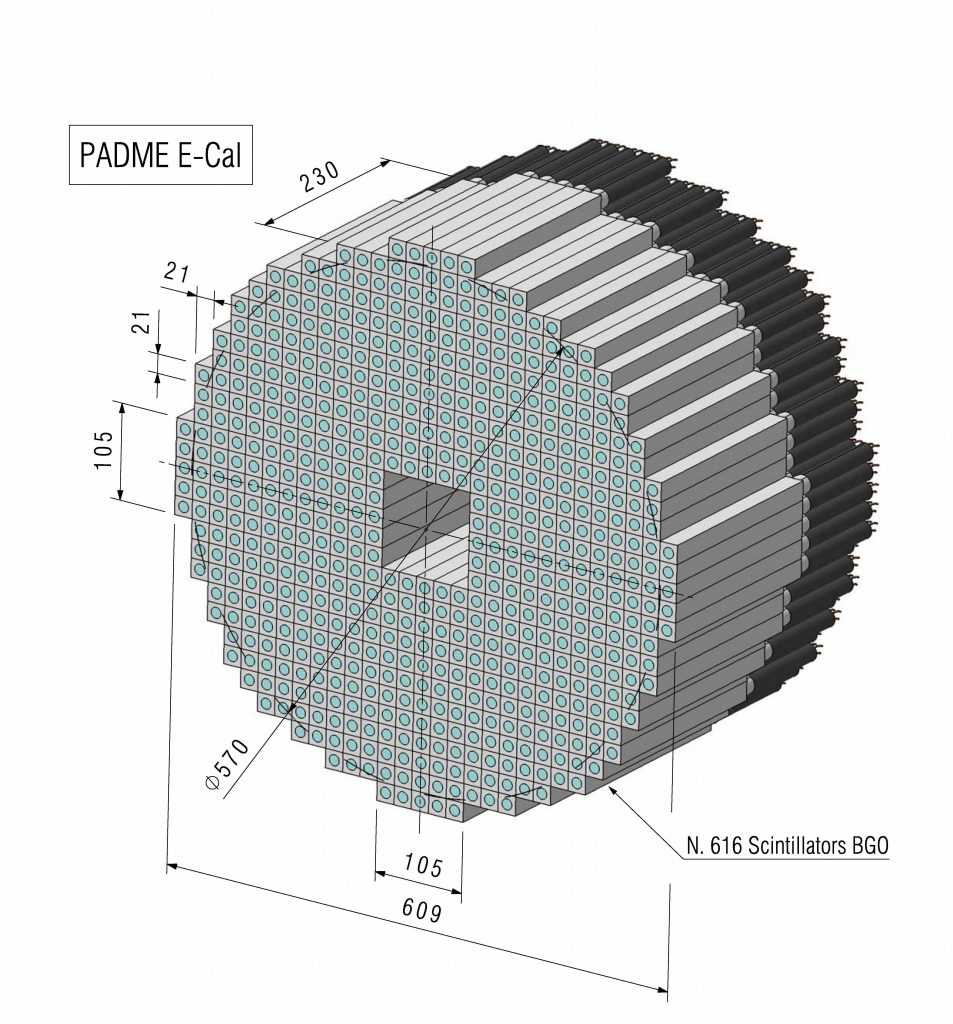
\includegraphics[width=0.9\textwidth]{graphics/ecal_big.jpg}
    \end{subfigure}%
    \begin{subfigure}{0.5\textwidth}
        \centering
        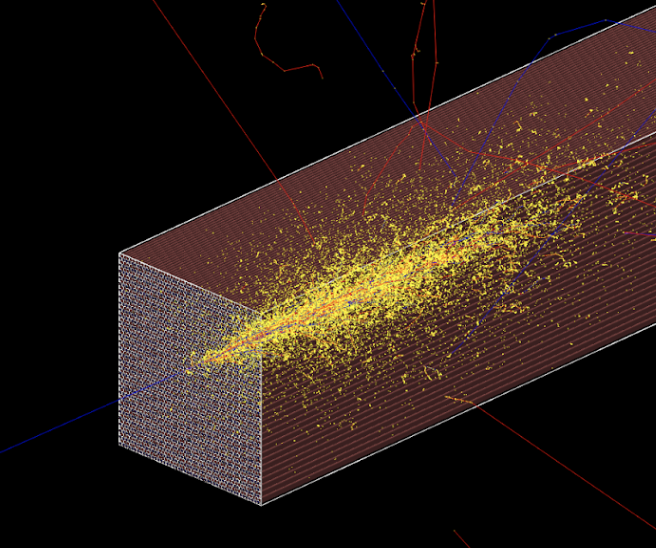
\includegraphics[width=0.9\textwidth]{graphics/shower.png}
    \end{subfigure}
    \caption[placeholder]{Электромагнитный калориметр PADME и симуляция электромагнитного ливня с помощью GEANT4\footnotemark.}
    \label{image:ecal}
\end{figure}

\footnotetext{Источники изображений: \url{https://padme.lnf.infn.it/ecal/} и \url{https://ep-news.web.cern.ch/content/geant4-modern-and-versatile-toolkit-detector-simulations}}

В этом исследовании мы изучаем оптимизацию размера датчика для экспериментов по физике элементарных частиц, сосредоточившись на реконструкции энергии и положения фотонов в ячейках электромагнитного калориметра. Мы предлагаем использовать методы глубинного обучения для решения этой задачи и оцениваем производительность калориметров, состоящих из чувствительных элементов в количестве от $10 \times 10$ до $40 \times 40$. В частности, мы обучаем модели глубинного обучения, включая сверточные нейронные сети (CNN), такие как ResNet18, и архитектуры на основе трансформеров, такие как Vision Transformer (ViT), для восстановления энергии и положения фотонов из смоделированных данных калориметра. Кроме того, мы сравниваем производительность этих моделей глубинного обучения с базовыми методами, такими как аналитическая модель и линейная регрессия (LinReg), учитывая такие метрики, как средняя квадратичная ошибка (MSE), средняя абсолютная ошибка (MAE), корневая средняя квадратичная ошибка (RMSE) и их взвешенные варианты.

Кроме того, мы изучаем влияние различных функций потерь, стратегий обучения и гиперпараметров моделей глубинного обучения на точность восстановления для датчиков разного размера. Систематически анализируя эти факторы, мы стремимся понять компромиссы, связанные с выбором оптимального размера датчика для электромагнитных калориметров в экспериментах по физике частиц. Наши выводы будут способствовать разработке и оптимизации будущих детекторных систем, позволяющих проводить более точные измерения свойств частиц с учетом практических ограничений и стоимости.

Оставшееся часть работы организована следующим образом. Раздел~\ref{section:related_work} рассказывают о существующих продвижениях в применении глубинного обучения для задач физики высоких энергий, а также приводит краткое описание используемых в данной работе моделей. В Разделе~\ref{section:method} подробно расписывается постановка решаемой задачи, приводится описание данных, используемые модели и техники. В Разделе~\ref{section:results} приводятся и обсуждаются результаты проведенных экспериментов. В Разделе~\ref{section:conclusion} мы подводим итоги наших выводов.

\colorbox{yellow}{Оформить гитхаб с документацией и комментариями}

Реализация всей процедуры обучения, а также проведения экспериментов доступны в интернете\footnote{\url{https://github.com/dxtvzw/ecal-optimization/tree/master/src}}.

\section{Обзор литературы}
\label{section:related_work}

\subsection{Смежные работы}
\label{subsection:related_work}

В области физики частиц наблюдается всплеск исследований, изучающих применение методов глубинного обучения для задач моделирования и реконструкции в экспериментах по физике высоких энергий. В работе~\cite{Belayneh_2020} были представлены алгоритмы глубинного обучения для моделирования и реконструкции калориметрии с использованием детального моделирования ливня в качестве обучающих данных. Их нейронная сеть для реконструкции, обученная на уровне калориметрических ячеек, продемонстрировала значительные улучшения по сравнению с современными алгоритмами, позволяя одновременно идентифицировать частицы и восстанавливать энергию. Эта работа очень актуальна для нашего исследования, поскольку мы также изучаем оптимизацию моделей глубокого обучения для реконструкции частиц в электромагнитных калориметрах, уделяя особое внимание оптимизации размера датчика и точности реконструкции.

Кроме того, в работе~\cite{Di_Bello_2021} предложен подход с использованием компьютерного зрения к алгоритмам Particle Flow (PFlow) в экспериментах по физике высоких энергий, использующий изображения калориметра для превосходной реконструкции энергетических распадов нейтральных частиц на фоне столкновения заряженных частиц. Их исследование продемонстрировало эффективность методов глубинного обучения в улучшении реконструкции кинематических свойств частиц, что соответствует нашей цели оптимизации размера датчика для улучшения пространственного разрешения и реконструкции энергии в электромагнитных калориметрах.

В смежном исследовании~\cite{PhysRevD.108.052002} представил новую методику, основанную на глубинном обучении, для реконструкции распадов частиц, усиленных преобразованием Лоренца, минуя традиционные аналитические методы реконструкции. Их подход, проверенный на данных о столкновениях на БАК, продемонстрировал замечательную производительность в восстановлении свойств частиц непосредственно из минимально обработанных данных детектора. Хотя основное внимание было уделено реконструкции распадов частиц, их методология и стратегии обучения актуальны для наших исследований по оптимизации размера датчика и точности реконструкции в электромагнитных калориметрах.

Кроме того, в работе~\cite{Akchurin_2021} сравнивалась производительность глубинных нейронных сетей, включая сверточные нейронные сети (CNN) и графовые нейронные сети (GNN), с современными методами восстановления энергии в сегментированных калориметрах. Сравнительный анализ показал значительное улучшение энергетического разрешения, достигнутое CNN, обученными на чистых образцах частиц, что подчеркивает важность скрытых представлений характеристик, используемых нейросетевыми методами. Это исследование дает ценное представление о потенциальных преимуществах подходов глубинного обучения для реконструкции энергии в калориметрах, что поможет нам в исследовании оптимизации размера датчика и точности реконструкции.

Наконец, в работе~\cite{Wemmer_2023} представлено исследование реконструкции фотонов в электромагнитном калориметре Belle II с помощью графовых нейронных сетей (GNN), демонстрирующее значительное улучшение энергетического разрешения по сравнению с существующими алгоритмами реконструкции. Их работа, сосредоточенная на восстановлении как изолированных, так и перекрывающихся фотонов, продемонстрировала многообещающий потенциал GNN в повышении энергетического разрешения и уменьшении хвостов в восстановленных энергетических распределениях. Это исследование совпадает с нашей исследовательской задачей по оптимизации размера датчика для улучшения реконструкции фотонов в электромагнитных калориметрах, что подчеркивает актуальность методов глубинного обучения для усовершенствования алгоритмов реконструкции частиц.

В целом, вышеупомянутые исследования подчеркивают растущий интерес к использованию методов глубинного обучения для задач моделирования и реконструкции в экспериментах по физике частиц, особенно в контексте калориметрии. Опираясь на идеи и методологии, представленные в этих работах, наше исследование призвано внести вклад в оптимизацию размеров датчиков для электромагнитных калориметров, что в конечном итоге повысит точность и эффективность реконструкции частиц в экспериментах по физике высоких энергий.

\subsection{Используемые методы}
\label{subsection:used_methods}

ResNet (Residual Neural Network) - это глубокая нейронная сеть, предназначенная для решения задач компьютерного зрения. Основная идея ResNet состоит в использовании блоков с остаточным соединением (residual connections), которые позволяют эффективно обучать глубокие сети, предотвращая проблему затухающего градиента.

Архитектура ResNet состоит из стека блоков, каждый из которых содержит несколько сверточных слоев. Важной особенностью ResNet является наличие skip-connections, которые позволяют пропускать через блок исходные признаки. Это позволяет избежать потери информации и упрощает обучение сети.

Принцип работы ResNet заключается в передаче информации через блоки с остаточным соединением, что помогает сети эффективно изучать более глубокие представления изображений. В процессе обучения, градиенты легче распространяются благодаря skip-connections, что способствует более стабильному и быстрому обучению сети.

Модель Vision Transformer (ViT) представляет собой архитектуру нейронной сети, разработанную для решения задач компьютерного зрения. Она основана на идее применения трансформеров, которые изначально были разработаны для обработки последовательностей, к обработке изображений.

Архитектура ViT состоит из двух основных компонентов: энкодера и классификатора. Энкодер состоит из нескольких слоев трансформера, включая механизм внимания (attention mechanism). Изображение разбивается на патчи, которые затем подаются на вход энкодеру. После обработки энкодером, полученные представления патчей объединяются и подаются на вход классификатору для выполнения задачи классификации. Можно заменить классификатор на регрессор и тогда модель будет решать задачи регрессии.

Одно из преимуществ ViT по сравнению с ResNet заключается в его способности эффективно обрабатывать изображения любого размера. В ResNet изображения обычно масштабируются до фиксированного размера, что может привести к потере информации или искажению изображения. В ViT изображение разбивается на патчи, поэтому размер изображения не ограничен, и модель может работать с изображениями различных размеров без необходимости их масштабирования.

Кроме того, ViT показывает хорошие результаты на ряде стандартных задач компьютерного зрения, демонстрируя сопоставимое или даже лучшее качество по сравнению с классическими архитектурами, такими как ResNet, при правильной настройке гиперпараметров и аугментации данных.

\section{Методология}
\label{section:method}

В этом Разделе мы описываем методику оптимизации размеров датчиков в электромагнитных калориметрах с помощью различных моделей глубокого обучения, включая аналитические модели, линейную регрессию, ResNet, простые сверточные сети и модели, основанные на архитектуре трансформеров.

\subsection{Данные}
\label{subsection:data}

Для данного исследования была использована следующая структура электромагнитного калориметра: результаты считывания замеров чувствительных элементов сенсора можно представить в виде матрицы $N \times N$ неотрицательных вещественных чисел, при этом сам калориметр состоит из $5 \times 5$ модулей. То есть если итоговая размерность калориметра это $40 \times 40$, это на самом деле значит, что он состоит из $5 \times 5$ модулей, каждый из которых разбит на $8 \times 8$ единичных ячеек. Физический размер всего сенсора калориметра это $60.6 \: \text{см} \times 60.6 \: \text{см}$. Увеличение количества ячеек означает уменьшение размера каждой отдельной ячейки. Набор данных состоит из смоделированных симуляций, представляющих взаимодействие одного фотона с электромагнитным калориметром. Всего для каждого размера сенсора имеется по $64'000$ примеров. Каждый элемент данных содержит такую информацию, как матрица неотрицательных значений (входные данные), а также положение входной точки фотона относительно центра сенсора и его соответствующая энергия в диапазоне от $1$ до $100$ ГэВ (целевые данные). Используя аналитические методы можно сделать сдвиг всей матрицы сенсора на необходимую позицию, что позволяет сделать предположение о том, что все фотоны прилетают в калориметр в его центральной клетке\footnote{В случае четной размерности сенсора и отсутствия центральной клетки, фотон сдвигался в правую нижнюю клетку, соседнюю с центром всего сенсора.}. На Рисунке~\ref{image:data_sample} показан пример входных данных и целевой позиции фотона. Симулирование данных было сделано с помощью инструмента GEANT4. В силу сложной структуры в которой хранятся результаты симуляций GEANT4, набор данных предварительно обрабатывался путем преобразования данных и их сохранения в виде Numpy массивов для ускорения загрузки во время обучения. Позиции входа фотонов для удобства нормализованы к диапазону $[0, 1]$. Значения энергии не нормируются и сохраняются в исходных единицах. Отношение обучающей и тестовой выборки выбрано равное $4$ к $1$.

\begin{figure}[t]
    \centering
    \begin{subfigure}{0.5\textwidth}
        \centering
        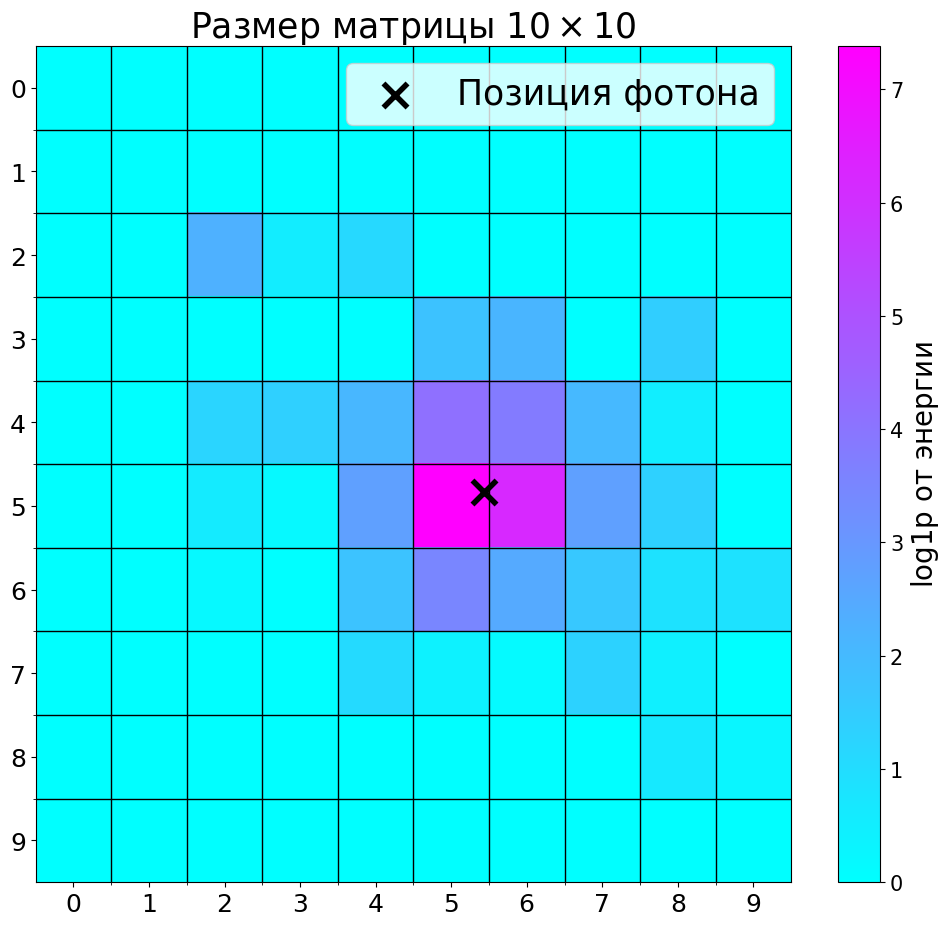
\includegraphics[width=0.9\textwidth]{graphics/data_10x10.png}
    \end{subfigure}%
    \begin{subfigure}{0.5\textwidth}
        \centering
        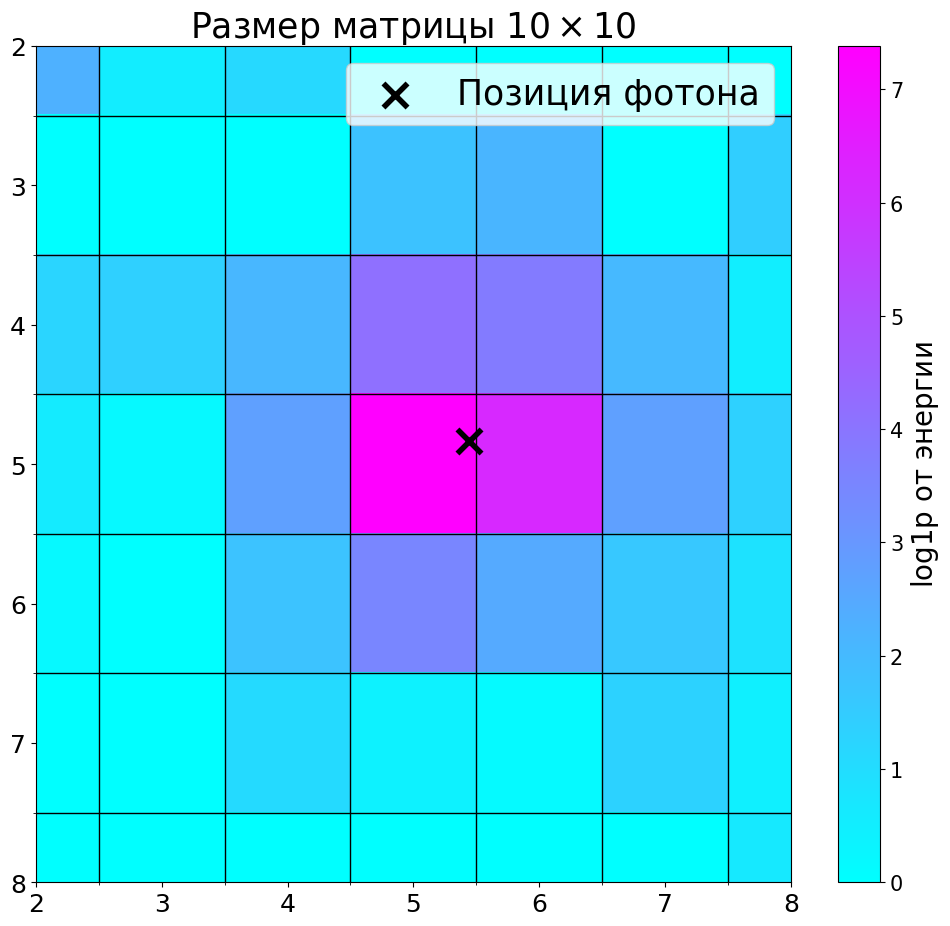
\includegraphics[width=0.9\textwidth]{graphics/data_10x10_zoomed.png}
    \end{subfigure}

    \begin{subfigure}{0.5\textwidth}
        \centering
        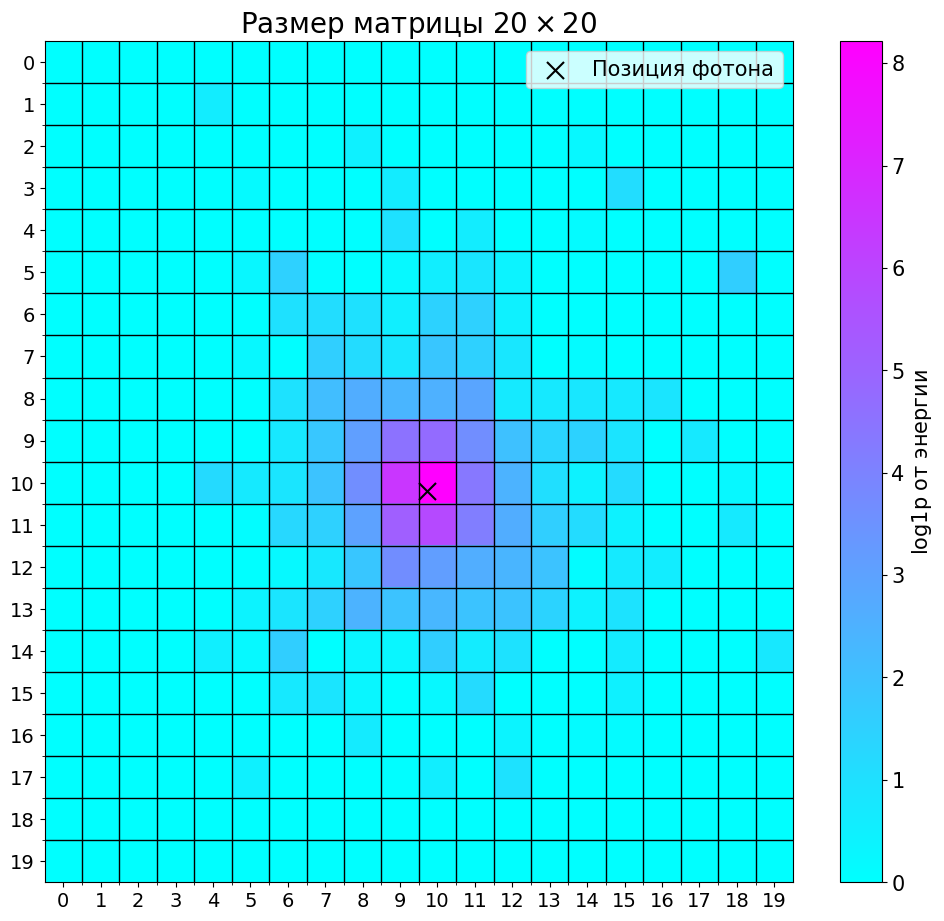
\includegraphics[width=0.9\textwidth]{graphics/data_20x20.png}
    \end{subfigure}%
    \begin{subfigure}{0.5\textwidth}
        \centering
        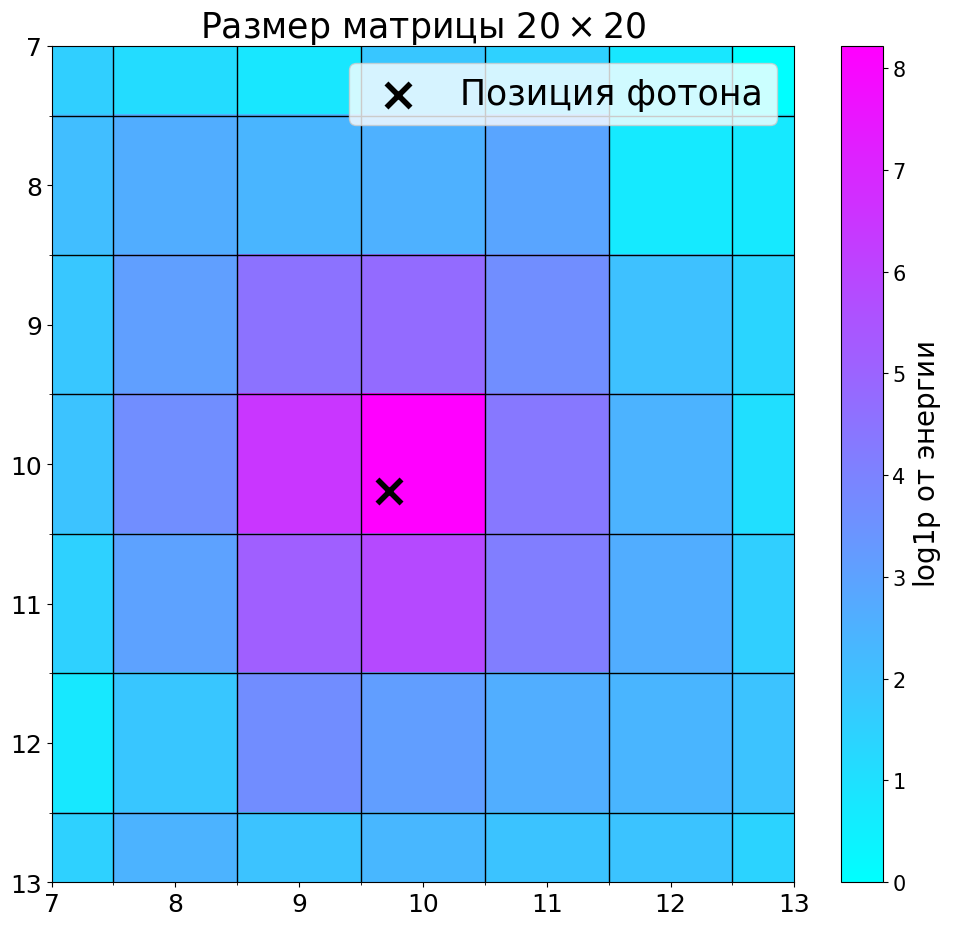
\includegraphics[width=0.9\textwidth]{graphics/data_20x20_zoomed.png}
    \end{subfigure}
    \caption{Примеры данных, считанных калориметром для разрешений $10 \times 10$ и $20 \times 20$. Слева показаны полноразмерные изображения, справа увеличенные центральные клетки. Настоящая позиция фотона обозначена черным крестиком. Для большей наглядности значения матриц показаны после применения функции $\mathsf{log1p} = \log(1 + x)$.}
    \label{image:data_sample}
\end{figure}

\subsection{Модели}

Несколько моделей глубинного обучения оцениваются на предмет их эффективности при реконструкции энергии и позиции для разных размеров датчиков:

\begin{itemize}
    \item \textbf{Аналитическая модель (AnaModel)}. Эта модель используют простые аналитические формулы для оценки целевых значений. Для задачи восстановления энергии она берет сумму значений всех ячеек матрицы и пропускает через один обучаемый линейный слой\footnote{Данный слой играет роль аффинного преобразования для подходящего выравнивания распределений.}. Для задачи реконструкции позиции модель создает в центре каждой ячейки калориметра точку с массой, равной значению считанной энергии данной ячейкой и вычисляет барицентр (центр масс) полученного множества взвешенных точек. Далее координаты полученной точки нормируются в нужный отрезок значений.
    \item \textbf{Линейная регрессия (LinReg)}. Модель линейной регрессии обучается предсказывать целевые значения на основе входных признаков. Данная модель состоит из одного единственного обучаемого слоя, переводящего все элементы матрицы в три вещественных числа (одно для энергии и два для позиции фотона).
    \item \textbf{ResNet18}. Описание данной модели можно найти в Разделе~\ref{subsection:used_methods}. У базовой архитектуры ResNet был удален первый слой, так как он был рассчитан на изображения размера $224 \times 224$, а в нашей задаче разрешение матриц сильно меньше и данный слой бы практически полностью терял информацию об исходных данных.
    \item \textbf{Простые сверточные сети (CNN)}. Базовые архитектуры сверточных нейронных сетей изучаются на предмет их способности извлекать пространственные признаки.
    \item \textbf{Vision Transformer (ViT)}. Рассматривается архитектура на основе трансформеров, адаптированная для задач зрения, чтобы использовать механизмы внимания для извлечения признаков (см. Раздел~\ref{subsection:used_methods}). Основным гиперпараметром модели является размер патча (patch size) на которые разбивается изображение, подающееся на вход модели. Было принято решение зафиксировать этот параметр равным $5$ (то есть каждая матрица входных данных разбивается на подматрицы размера $5 \times 5$), потому что модель требует целочисленной делимости размера изображения на размер патча, а в нашей задаче по построению калориметр состоит из $5 \times 5$ модулей, а значит разрешение калориметра всегда делится на $5$.
\end{itemize}

Современные модели глубинного обучения типично состоят из двух частей: основное тело (backbone) и голова (prediction head). Тело модели отвечает за извлечение сложных и показательных признаков из данных, а голова необходима для, собственно, решения задачи основываясь на этих полученных признаках. В данной работе предлагается одновременное решение поставленных задач (реконструкция энергии и реконструкция позиции фотона) с помощью добавления дополнительной головы к вышеуказанным моделям.

\subsection{Процедура обучения}

Выбранные модели обучаются на подготовленном наборе данных. Процесс обучения включает в себя оптимизацию параметров модели для минимизации комбинированной функции потерь, которая представляет собой взвешенную сумму двух отдельных потерь: одной для восстановления энергии и другой для восстановления положения фотонов. Коэффициенты взвешенной суммы варьируются в разных экспериментах для изучения их влияния на производительность. Обучение проводилось с использованием оптимизатора AdamW, базовой длиной шага (learning rate) $0.007$ и нулевым сокращением веса (weight decay). Использовалось косинусное расписание с прогревом (linear warmup with cosine annealing). Модели обучались в течение $100$ эпох включая $15$ эпох на прогрев расписания. Размер подвыборки (batch size) для шага оптимизации во всех экспериментах был $512$.

\subsection{Метрики качества}
\label{subsection:metrics}

В данном исследовании рассматривались следующие функции потерь: Предположим, что дана выборка данных $(x_i, y_i)_{i = 1}^{n}$, где $x_i$ --- входные данные и $y_i$ --- целевые значения. Далее пусть $\{ a_i \}_{i = 1}^{n}$ предсказания модели для этих данных. Тогда

\begin{itemize}
    \item Корень из среднеквадратичной ошибки (\textsf{RMSE}): \[ \textsf{RMSE}(a, y) = \sqrt{\frac{1}{n} \sum_{i = 1}^{n} (a_i - y_i)^2} . \]
    \item Средняя абсолютная ошибка (\textsf{MAE}): \[ \textsf{MAE}(a, y) = \frac{1}{n} \sum_{i = 1}^{n} |a_i - y_i| . \]
    \item Корень из среднеквадратичной логирифмической ошибки (\textsf{RMSLE}): \[ \textsf{RMSLE}(a, y) = \sqrt{\frac{1}{n} \sum_{i = 1}^{n} (\log(a_i + 1) - \log(y_i + 1))^2} . \]
    \item Взвешенный корень из среднеквадратичной ошибки (\textsf{RMSE/E}): \[ \textsf{RMSE/E}(a, y) = \sqrt{\frac{1}{n} \sum_{i = 1}^{n} \left( \frac{a_i - y_i}{y_i} \right)^2} . \]
    \item Взвешенная средняя абсолютная ошибка (\textsf{MAE/E}): \[ \textsf{MAE/E}(a, y) = \frac{1}{n} \sum_{i = 1}^{n} \frac{|a_i - y_i|}{y_i} . \]
\end{itemize}

В качестве метрик итогового качества для реконструкции энергии и позиции были выбраны $\mathcal{L}_{\mathsf{eng}} = \textsf{RMSE/E}$ и $\mathcal{L}_{\mathsf{pos}} = \textsf{RMSE}$ соответственно. Эти же две функции используются как функции потерь для соответствующих задач если не сказано иное, а именно итоговой функцией обучения будет \begin{equation}\label{eq:loss_total}
    \mathcal{L}_{\mathsf{total}} = \alpha \cdot \mathcal{L}_{\mathsf{eng}} + (1 - \alpha) \cdot \mathcal{L}_{\mathsf{pos}}
\end{equation} где $\alpha \in [0, 1]$ --- гиперпараметр важности той или иной задачи\footnote{Увеличение $\alpha$ дает больший приоритет задаче восстановления энергии, в то время как уменьшение $\alpha$ способствует лучшему решению задачи реконструкции позиции.}. Дополнительно, через $\mathcal{L}_{\mathsf{total}}^{\mathsf{train}}, \mathcal{L}_{\mathsf{eng}}^{\mathsf{train}}, \mathcal{L}_{\mathsf{pos}}^{\mathsf{train}}$ и $\mathcal{L}_{\mathsf{total}}^{\mathsf{val}}, \mathcal{L}_{\mathsf{eng}}^{\mathsf{val}}, \mathcal{L}_{\mathsf{pos}}^{\mathsf{val}}$ будем обозначать значение данных метрик на обучающей и валидационной (тестовой) выборках соответственно. По умолчанию везде будет считаться, что $\mathcal{L}_{\mathsf{total}} = \mathcal{L}_{\mathsf{total}}^{\mathsf{val}}, \mathcal{L}_{\mathsf{eng}} = \mathcal{L}_{\mathsf{eng}}^{\mathsf{val}}$ и $\mathcal{L}_{\mathsf{pos}} = \mathcal{L}_{\mathsf{pos}}^{\mathsf{val}}$.

Выбор взвешенной метрики \textsf{RMSE/E} для реконструкции энергии обоснован важностью относительной погрешности по сравнению с абсолютной погрешностью в экспериментах по физике высоких энергий. Относительная ошибка учитывает пропорциональное расхождение между предсказанными и фактическими значениями энергии, что имеет решающее значение для поддержания точности в широком диапазоне уровней энергии. В экспериментах, связанных со столкновениями частиц, где измерения энергии имеют фундаментальное значение для понимания свойств и взаимодействия частиц, точная количественная оценка относительных отклонений необходима для точного анализа и интерпретации. Поэтому, взвешивая метрику \textsf{RMSE/E}, мы отдаем приоритет относительной точности реконструкции энергии, обеспечивая надлежащий масштаб расхождений по отношению к величине энергии, тем самым повышая общую надежность и интерпретируемость результатов.

Выбор метрики \textsf{RMSE} для реконструкции позиции обоснован тем, что эта метрика совпадает с евклидовым расстоянием на плоскости (с точностью до мультипликативной константы) и является естественным показателем качества.

Во всех метриках чем меньше получаемое значение, тем лучше, при этом минимальное возможное значение ограничено $0$.

\subsection{Аугментации}
\label{subsection:augmentations}

В ходе исследования было принято решение использовать аугментации данных для улучшения качества моделей глубинного обучения. Аугментация данных --- это процесс модификации имеющихся данных путем применения различных трансформаций, таких как повороты и отражения, с целью увеличения разнообразия обучающей выборки и улучшения обобщающей способности моделей.

Одной из примененных аугментаций было случайное горизонтальное или вертикальное отражение матрицы калориметра. Это позволяет модели обучаться на различных вариантах изображений фотона, которые могут встречаться в реальных условиях эксперимента. При этом точка, представляющая позицию фотона в центральной клетке калориметра, также подвергается отражению в соответствии с производимой трансформацией, чтобы сохранить соответствие между позицией фотона и его отражением.

Другой примененной аугментацией был случайный поворот матрицы калориметра на углы вида $0^{\circ}$, $90^{\circ}$, $180^{\circ}$ и $270^{\circ}$. Эта трансформация позволяет модели обучаться на различных ориентациях фотона в калориметре и учитывать различные варианты расположения позиции фотона. Важно отметить, что при повороте матрицы точка в центральной клетке также подвергается повороту на соответствующий угол, чтобы корректно отобразить новое положение фотона после поворота. Поворот применялся только на углы, кратные $90^{\circ}$ для того, чтобы физический поворот сенсора переводил его в себя без лишних перекрытий и выходов за границы.

Использование указанных аугментаций позволяет обогатить обучающий набор данных и сделать модели более устойчивыми к различным вариантам входных данных, что в свою очередь способствует улучшению их обобщающей способности и точности реконструкции энергии и позиции фотона в электромагнитном калориметре.

\subsection{Постановка экспериментов}

Были проведены множественные эксперименты, включающие в себя сравнение различных архитектур моделей на всех имеющихся размерах сенсоров, сравнение эффективности функций потерь, влияние сложности модели и аугментации данных на итоговое качество.

Для более качественного сравнения во всех экспериментах были зафиксированы все источники случайности, кроме инициализации весов-параметров моделей, а также случайности компьютерных компонент. Замеры для каждого эксперимента проводились по $8$ раз и в качестве итогового результата бралось медианное значение.

\subsection{Ресурсы}

Для проведения экспериментов использовался кластер с AMD EPYC 9354 CPU и восемью RTX4090 GPU. Суммарное время исполнения всех экспериментов оценивается в $90$ часов.

\subsection{Анализ результатов}

Результаты, полученные в ходе экспериментов, анализируются с целью выявления наиболее эффективной модели и конфигурации для оптимизации размеров датчиков в электромагнитных калориметрах. Также исследуется влияние различных размеров датчиков на энергию и точность восстановления положения.

\section{Результаты}
\label{section:results}

В этом Разделе мы представляем результаты экспериментов по оптимизации размеров датчиков в электромагнитных калориметрах с использованием различных моделей глубинного обучения. Результаты анализируются на основе метрик качества, определенных в Разделе~\ref{subsection:metrics}.

Сперва было проведено сравнение качества различных моделей на всех имеющихся размерах сенсоров. Как показывает Таблица~\ref{table:all_models}, аналитическая модель, а также линейная регрессия уже дают достаточно хорошее качество реконструкции энергии фотонов, но при этом сильно отстают в восстановлении позиции. Стоит заметить, что аналитическая модель получает лучшее качество в реконструкции позиции, чем линейная регрессия, потому что она по построению учитывает физическое расположение ячеек сенсора. Модель \textsf{ResNet18} оказывается слишком сложной для маленьких размеров сенсоров и сильно проигрывает даже аналитической модели, но при этом показывает весьма хорошие результаты на сенсорах более высокого разрешения. Намного более простой сверточной нейронной сети \textsf{CNN} удается получить приемлемые результаты на сенсорах меньшего разрешения, но она не справляется с задачей реконструкции позиции на некоторых из размеров сенсоров. Единственная архитектура, которая показывает отличные результаты на обоих задачах и всех размерах сенсоров оказывается \textsf{ViT}, поэтому во всех последующих экспериментах анализировалась именно данная модель.

\begin{table}[t]
	\footnotesize
	\centering
	\begin{tabular}{llrrrrrrr}
		\toprule
		{} & {} & \multicolumn{6}{c}{\textsf{Размер матрицы}} \\
		\cmidrule(lr){3-8}
		\textsf{Модель} & \textsf{Метрика} & $\mathsf{10 \times 10}$ &  $\mathsf{15 \times 15}$ &  $\mathsf{20 \times 20}$ &  $\mathsf{25 \times 25}$ &  $\mathsf{30 \times 30}$ &  $\mathsf{40 \times 40}$ \\
		\midrule
        \textsf{AnaModel} & $\mathcal{L}_{\mathsf{total}}$ & $\mathsf{0.0626}$ & $\mathsf{0.0518}$ & $\mathsf{0.0469}$ & $\mathsf{0.0448}$ & $\mathsf{0.0440}$ & $\mathsf{0.0467}$ \\
        {} & $\mathcal{L}_{\mathsf{eng}}$ & $\mathsf{0.0213}$ & $\mathsf{0.0221}$ & $\mathsf{0.0226}$ & $\mathsf{0.0229}$ & $\mathsf{0.0220}$ & $\mathsf{0.0222}$ \\
        {} & $\mathcal{L}_{\mathsf{pos}}$ & $\mathsf{0.1040}$ & $\mathsf{0.0817}$ & $\mathsf{0.0714}$ & $\mathsf{0.0670}$ & $\mathsf{0.0662}$ & $\mathsf{0.0716}$ \\
        \midrule
        \textsf{LinReg} & $\mathcal{L}_{\mathsf{total}}$ & $\mathsf{0.0728}$ & $\mathsf{0.0738}$ & $\mathsf{0.0741}$ & $\mathsf{0.0745}$ & $\mathsf{0.0748}$ & $\mathsf{0.0751}$ \\
        {} & $\mathcal{L}_{\mathsf{eng}}$ & $\mathsf{0.0213}$ & $\mathsf{0.0221}$ & $\mathsf{0.0226}$ & $\mathsf{0.0231}$ & $\mathsf{0.0221}$ & $\mathsf{0.0223}$ \\
        {} & $\mathcal{L}_{\mathsf{pos}}$ & $\mathsf{0.1244}$ & $\mathsf{0.1258}$ & $\mathsf{0.1257}$ & $\mathsf{0.1264}$ & $\mathsf{0.1278}$ & $\mathsf{0.1282}$ \\
        \midrule
        \textsf{Resnet18} & $\mathcal{L}_{\mathsf{total}}$ & $\mathsf{0.0926}$ & $\mathsf{0.0823}$ & $\mathsf{0.0248}$ & $\mathsf{0.0254}$ & $\mathsf{0.0707}$ & $\mathsf{0.0271}$ \\
        {} & $\mathcal{L}_{\mathsf{eng}}$ & $\mathsf{0.0814}$ & $\mathsf{0.0705}$ & $\mathsf{0.0215}$ & $\mathsf{0.0215}$ & $\mathsf{0.0565}$ & $\mathsf{0.0207}$ \\
        {} & $\mathcal{L}_{\mathsf{pos}}$ & $\mathsf{0.1042}$ & $\mathsf{0.0941}$ & $\mathsf{0.0284}$ & $\mathsf{0.0297}$ & $\mathsf{0.0851}$ & $\mathsf{0.0336}$ \\
        \midrule
        \textsf{CNN} & $\mathcal{L}_{\mathsf{total}}$ & $\mathsf{0.0229}$ & $\mathsf{0.0240}$ & $\mathsf{0.0682}$ & $\mathsf{0.5922}$ & $\mathsf{0.0260}$ & $\mathsf{0.1326}$ \\
        {} & $\mathcal{L}_{\mathsf{eng}}$ & $\mathsf{0.0197}$ & $\mathsf{0.0200}$ & $\mathsf{0.0201}$ & $\mathsf{0.8934}$ & $\mathsf{0.0197}$ & $\mathsf{0.0196}$ \\
        {} & $\mathcal{L}_{\mathsf{pos}}$ & $\mathsf{0.0262}$ & $\mathsf{0.0281}$ & $\mathsf{0.1166}$ & $\mathsf{0.2912}$ & $\mathsf{0.0324}$ & $\mathsf{0.2462}$ \\
        \midrule
        \textsf{ViT} & $\mathcal{L}_{\mathsf{total}}$ & $\mathsf{0.0221}$ & $\mathsf{0.0232}$ & $\mathsf{0.0243}$ & $\mathsf{0.0242}$ & $\mathsf{0.0253}$ & $\mathsf{0.0264}$ \\
        {} & $\mathcal{L}_{\mathsf{eng}}$ & $\mathsf{0.0194}$ & $\mathsf{0.0198}$ & $\mathsf{0.0203}$ & $\mathsf{0.0194}$ & $\mathsf{0.0196}$ & $\mathsf{0.0193}$ \\
        {} & $\mathcal{L}_{\mathsf{pos}}$ & $\mathsf{0.0250}$ & $\mathsf{0.0270}$ & $\mathsf{0.0285}$ & $\mathsf{0.0295}$ & $\mathsf{0.0311}$ & $\mathsf{0.0336}$ \\
        
		\bottomrule
	\end{tabular}
    \caption{Сравнение качества моделей на различных размерах сенсоров. Каждая модель независимо обучалась для каждого размера сенсоров на обе задачи реконструкции одновременно.}
	\label{table:all_models}
\end{table}

Улучшение производительности, наблюдаемое при использовании более сложных моделей, таких как \textsf{ResNet18} и \textsf{ViT}, подчеркивает важность использования сложности модели для улавливания сложных закономерностей в данных. Эти модели обладают большей репрезентативной способностью, что позволяет им изучать иерархические особенности и глубокие зависимости, которые имеют решающее значение для точной реконструкции энергии и положения. В отличие от исключительно сверточных нейронных сетей, которые полагаются только на локальные рецептивные поля, Vision Transformers используют механизмы внимания для улавливания взаимодействий между удаленными областями калориметра. Это позволяет модели учитывать контекстную информацию из всего пространства входных данных, что приводит к принятию более обоснованных решений.

Далее было проведено сравнение качества обучения модели \textsf{ViT} на различные функции потерь для реконструкции энергии (функция потерь для восстановления позиции оставалась изначальной $\mathcal{L}_{\textsf{pos}} = \textsf{RMSE}$). Из Таблицы~\ref{table:loss_comp} можно видеть, что все нормализованные\footnote{устойчивые к изменению магнитуды целевых значений} функции потерь \textsf{RMSE/E}, \textsf{MAE/E} и \textsf{RMSLE} приводят к заметно лучшим результатам, чем ненормализованная функция потерь \textsf{RMSE}. Более того, Рисунок~\ref{graph:loss_distr} показывает, что наибольшие значения метрики качества (на графике показана метрика \textsf{MAE/E}) получаются на данных с наименьшими значениями энергии, при этом функция потерь \textsf{RMSE/E} приводит к более равномерному распределению, чем \textsf{RMSE}.

\begin{table}[t]
	\footnotesize
	\centering
	\begin{tabular}{llrrrrrrr}
		\toprule
		{} & {} & \multicolumn{6}{c}{\textsf{Размер матрицы}} \\
		\cmidrule(lr){3-8}
		\textsf{Функция потерь} & \textsf{Метрика} & $\mathsf{10 \times 10}$ &  $\mathsf{15 \times 15}$ &  $\mathsf{20 \times 20}$ &  $\mathsf{25 \times 25}$ &  $\mathsf{30 \times 30}$ &  $\mathsf{40 \times 40}$ \\
		\midrule
        \textsf{RMSE/E} & $\mathcal{L}_{\mathsf{eng}}$ & $\mathsf{0.0194}$ & $\mathsf{0.0198}$ & $\mathsf{0.0201}$ & $\mathsf{0.0192}$ & $\mathsf{0.0193}$ & $\mathsf{0.0195}$ \\
        {} & $\mathcal{L}_{\mathsf{pos}}$ & $\mathsf{0.0250}$ & $\mathsf{0.0269}$ & $\mathsf{0.0284}$ & $\mathsf{0.0294}$ & $\mathsf{0.0310}$ & $\mathsf{0.0338}$ \\
        \midrule
        \textsf{MAE/E} & $\mathcal{L}_{\mathsf{eng}}$ & $\mathsf{0.0198}$ & $\mathsf{0.0200}$ & $\mathsf{0.0204}$ & $\mathsf{0.0199}$ & $\mathsf{0.0199}$ & $\mathsf{0.0200}$ \\
        {} & $\mathcal{L}_{\mathsf{pos}}$ & $\mathsf{0.0251}$ & $\mathsf{0.0269}$ & $\mathsf{0.0284}$ & $\mathsf{0.0294}$ & $\mathsf{0.0312}$ & $\mathsf{0.0336}$ \\
        \midrule
        \textsf{RMSLE} & $\mathcal{L}_{\mathsf{eng}}$ & $\mathsf{0.0193}$ & $\mathsf{0.0196}$ & $\mathsf{0.0204}$ & $\mathsf{0.0191}$ & $\mathsf{0.0194}$ & $\mathsf{0.0194}$ \\
        {} & $\mathcal{L}_{\mathsf{pos}}$ & $\mathsf{0.0249}$ & $\mathsf{0.0269}$ & $\mathsf{0.0285}$ & $\mathsf{0.0294}$ & $\mathsf{0.0310}$ & $\mathsf{0.0338}$ \\
        \midrule
        \textsf{RMSE} & $\mathcal{L}_{\mathsf{eng}}$ & $\mathsf{0.0222}$ & $\mathsf{0.0222}$ & $\mathsf{0.0238}$ & $\mathsf{0.0214}$ & $\mathsf{0.0216}$ & $\mathsf{0.0219}$ \\
        {} & $\mathcal{L}_{\mathsf{pos}}$ & $\mathsf{0.0290}$ & $\mathsf{0.0294}$ & $\mathsf{0.0332}$ & $\mathsf{0.0363}$ & $\mathsf{0.0356}$ & $\mathsf{0.0385}$ \\
		\bottomrule
	\end{tabular}
    \caption{Сравнение обучения модели \textsf{ViT} при различных функциях потерь для задачи реконструкции энергии фотона. Метрики качества остаются такими же, как было определено в Разделе~\ref{subsection:metrics}.}
	\label{table:loss_comp}
\end{table}

\begin{figure}[t]
    \centering
    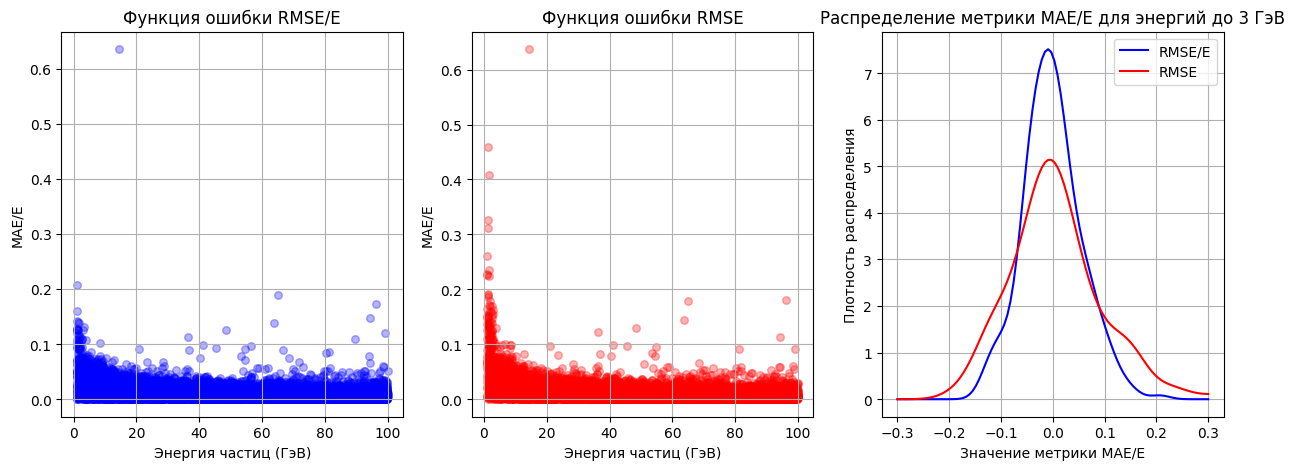
\includegraphics[width=1.0\textwidth]{graphics/exp2_distr_comp.png}
    \caption{Сравнение распределения метрики \textsf{MAE/E} на тестовых данных для модели \textsf{ViT}, обученной с помощью одной из двух функций потерь \textsf{RMSE/E} и \textsf{RMSE} в задаче реконструкции энергии.}
    \label{graph:loss_distr}
\end{figure}

Следующим объектом исследования был гиперпараметр $\alpha$ из выражения~(\ref{eq:loss_total}), отвечающий за отношение функций потерь двух задач в итоговой функции потерь. Исходя из Рисунка~\ref{graph:alpha} можно заметить, что качество на задачах реконструкции энергии и реконструкции позиции и вправду ведет себя так же, как и соответствующее изменение гиперпараметра $\alpha$ (больший вес в функции потерь приводит к лучшему качеству на данной задаче). Также получается, что взятие $\alpha = 0.5$ приводит к лучшим результатам в совокупности двух задач. Также посмотрев на крайние значения $\alpha$\footnote{На графиках не были указаны граничные случаи $\alpha = 0$ и $\alpha = 1$ потому что при данных значениях одна из функций потерь не обучалась вовсе и достигала слишком больших значений, что мешало визуальному сравнению более содержательных не граничных значений $\alpha$.} видно, что обучение модели на обе задачи одновременно практически никак не сказывается на результатах в каждой задаче отдельно.

\begin{figure}[t]
    \centering
    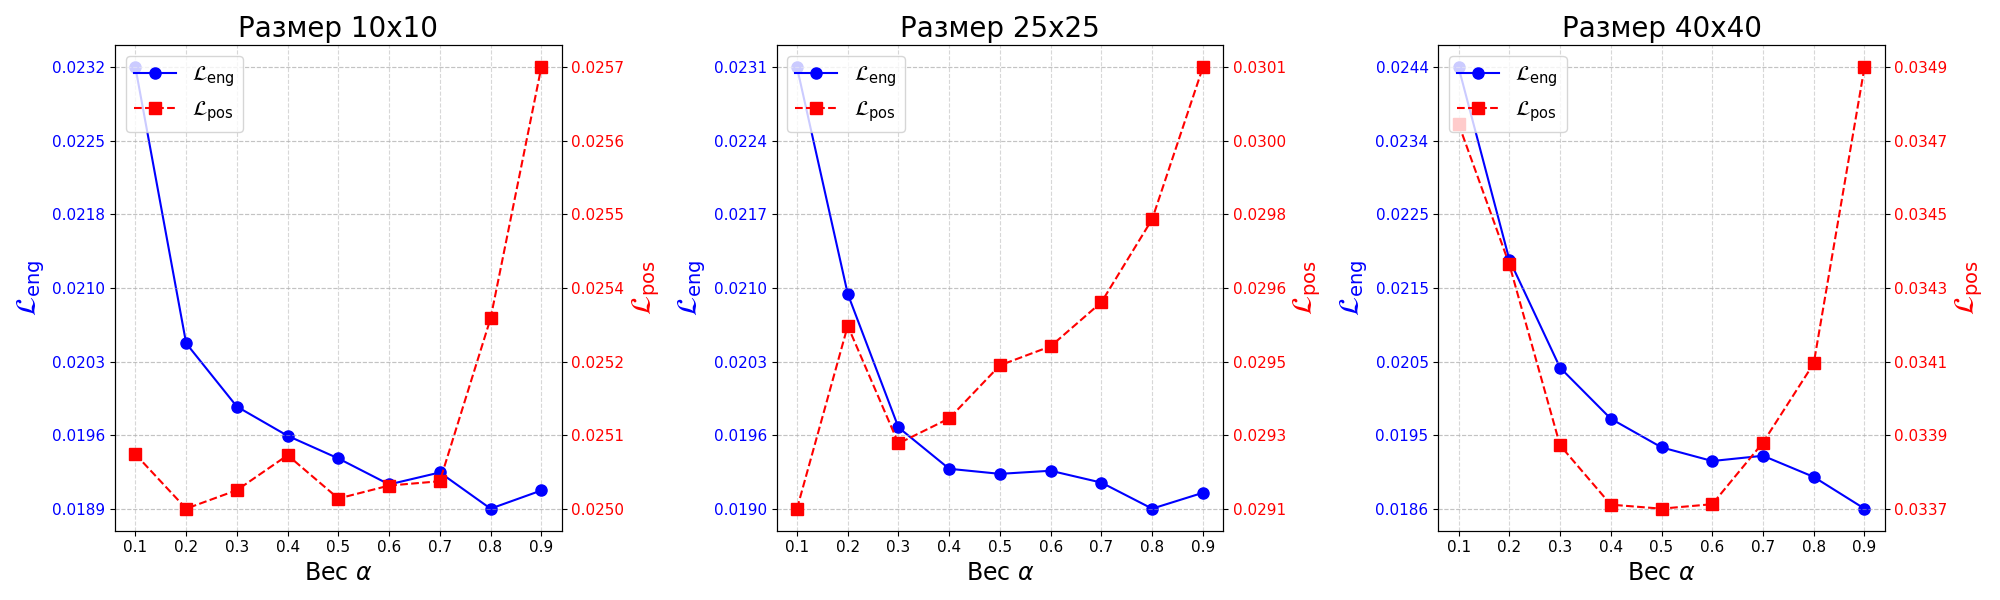
\includegraphics[width=1.0\textwidth]{graphics/exp3_alpha.png}
    \caption{Сравнение метрик качества модели \textsf{ViT} при подборе гиперпараметра $\alpha$ из выражения функции потерь~(\ref{eq:loss_total}).}
    \label{graph:alpha}
\end{figure}

Очередным экспериментом было сравнение влияния размера модели на качество решения задач. На Рисунке~\ref{graph:model_params} можно видеть, что чрезмерное увеличение размера модели плохо влияет на качество реконструкции позиции фотона, при этом качество восстановления энергии лишь немного ухудшается с увеличением размера модели. С другой стороны, слишком маленькие модели не способны выучиться решать задачу восстановления энергии.

\begin{figure}[t]
    \centering
    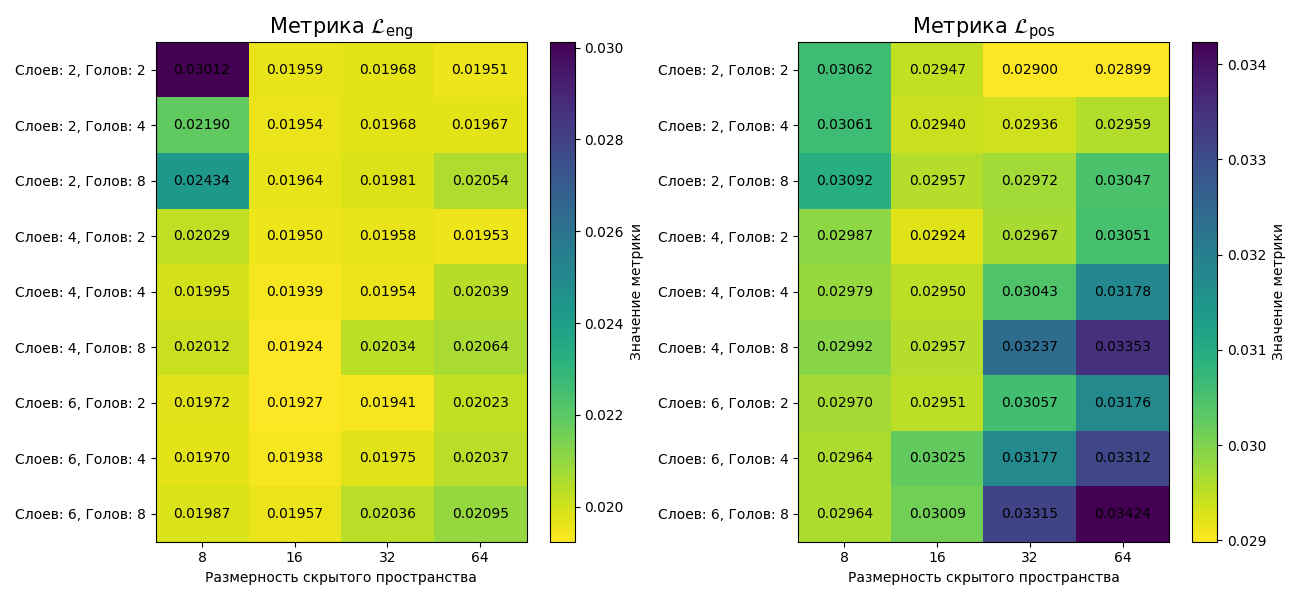
\includegraphics[width=1.0\textwidth]{graphics/exp4_model_params.png}
    \caption{Сравнение качества модели \textsf{ViT} на сенсоре размера $25 \times 25$ при изменении её параметров, таких как количество слоев, голов и размерность скрытого пространства (размерность MLP слоев была ровно в $4$ раза больше размерности скрытого пространства).}
    \label{graph:model_params}
\end{figure}

Последним предметом экспериментов стало сравнение влияния аугментаций на итоговое качество модели. Судя по Таблице~\ref{table:augmentations}, применение аугментаций заметно улучшает качество для сенсоров размера $15 \times 15$ и немного для размера $25 \times 25$. Более того, для обоих размеров аугментации приводят к сужению разрыва между качеством модели на обучающей и валидационной выборке, что показывает эффективность применяемых трансформаций.

\begin{table}[t]
	\footnotesize
	\centering
	\begin{tabular}{cc|cccc|cccc}
		\toprule
		{} & {} & \multicolumn{8}{c}{\textsf{Размер матрицы}} \\
		\cmidrule(lr){3-10}
        {} & {} & \multicolumn{4}{c}{$\mathsf{15 \times 15}$} \vline & \multicolumn{4}{c}{$\mathsf{25 \times 25}$} \\
		\midrule
        \textsf{Отражения} & \textsf{Повороты} & $\mathcal{L}_{\mathsf{eng}}^{\mathsf{train}}$ & $\mathcal{L}_{\mathsf{pos}}^{\mathsf{train}}$ & $\mathcal{L}_{\mathsf{eng}}^{\mathsf{val}}$ & $\mathcal{L}_{\mathsf{pos}}^{\mathsf{val}}$ & $\mathcal{L}_{\mathsf{eng}}^{\mathsf{train}}$ & $\mathcal{L}_{\mathsf{pos}}^{\mathsf{train}}$ & $\mathcal{L}_{\mathsf{eng}}^{\mathsf{val}}$ & $\mathcal{L}_{\mathsf{pos}}^{\mathsf{val}}$ \\
        \midrule
        \xmark & \xmark & $\mathsf{0.0182}$ & $\mathsf{0.0255}$ & $\mathsf{0.0217}$ & $\mathsf{0.0269}$ & $\mathsf{0.0181}$ & $\mathsf{0.0291}$ & $\mathsf{0.0192}$ & $\mathsf{0.0294}$ \\
        \cmark & \xmark & $\mathsf{0.0186}$ & $\mathsf{0.0259}$ & $\mathsf{0.0194}$ & $\mathsf{0.0269}$ & $\mathsf{0.0186}$ & $\mathsf{0.0295}$ & $\mathsf{0.0191}$ & $\mathsf{0.0293}$ \\
        \xmark & \cmark & $\mathsf{0.0185}$ & $\mathsf{0.0258}$ & $\mathsf{0.0193}$ & $\mathsf{0.0267}$ & $\mathsf{0.0186}$ & $\mathsf{0.0296}$ & $\mathsf{0.0189}$ & $\mathsf{0.0293}$ \\
        \cmark & \cmark & $\mathsf{0.0185}$ & $\mathsf{0.0258}$ & $\mathsf{0.0192}$ & $\mathsf{0.0267}$ & $\mathsf{0.0186}$ & $\mathsf{0.0295}$ & $\mathsf{0.0189}$ & $\mathsf{0.0292}$ \\
        
		\bottomrule
	\end{tabular}
    \caption{Сравнение качества модели \textsf{ViT} при применении различных аугментаций (см. Раздел~\ref{subsection:augmentations}).}
	\label{table:augmentations}
\end{table}

\begin{table}[t]
	\footnotesize
	\centering
	\begin{tabular}{lrrrrrrr}
		\toprule
		{} & \multicolumn{6}{c}{\textsf{Размер матрицы}} \\
		\cmidrule(lr){2-7}
		\textsf{Метрика} & $\mathsf{10 \times 10}$ &  $\mathsf{15 \times 15}$ &  $\mathsf{20 \times 20}$ &  $\mathsf{25 \times 25}$ &  $\mathsf{30 \times 30}$ &  $\mathsf{40 \times 40}$ \\
        \midrule
        $\mathcal{L}_{\mathsf{total}}$ & $\mathsf{0.0219}$ & $\mathsf{0.0227}$ & $\mathsf{0.0239}$ & $\mathsf{0.0237}$ & $\mathsf{0.0249}$ & $\mathsf{0.0262}$ \\
        $\mathcal{L}_{\mathsf{eng}}$ & $\mathsf{0.0189}$ & $\mathsf{0.0189}$ & $\mathsf{0.0194}$ & $\mathsf{0.0187}$ & $\mathsf{0.0189}$ & $\mathsf{0.0190}$ \\
        $\mathcal{L}_{\mathsf{pos}}$ & $\mathsf{0.0247}$ & $\mathsf{0.0265}$ & $\mathsf{0.0283}$ & $\mathsf{0.0289}$ & $\mathsf{0.0308}$ & $\mathsf{0.0334}$ \\
        $\textsf{MAE/E}_{\textsf{eng}}$ & $\mathsf{0.0131}$ & $\mathsf{0.0127}$ & $\mathsf{0.0132}$ & $\mathsf{0.0124}$ & $\mathsf{0.0130}$ & $\mathsf{0.0129}$ \\
        $\overline{\mathcal{L}}_{\mathsf{pos}}$ & $\mathsf{0.2117}$ & $\mathsf{0.1515}$ & $\mathsf{0.1211}$ & $\mathsf{0.0989}$ & $\mathsf{0.0881}$ & $\mathsf{0.0715}$ \\
        \textsf{Размер одной ячейки} & $\mathsf{6.0600}$ & $\mathsf{4.0400}$ & $\mathsf{3.0300}$ & $\mathsf{2.4240}$ & $\mathsf{2.0200}$ & $\mathsf{1.5150}$ \\           
        \bottomrule
	\end{tabular}
    \caption{Лучшее качество модели \textsf{ViT} на всех размерах сенсоров. Размер одной ячейки калориметра измеряется в сантиметрах. $\overline{\mathcal{L}}_{\mathsf{pos}}$ --- величина $\mathcal{L}_{\mathsf{pos}}$, переведенная в сантиметры для сравнения с общей величиной центральной ячейки (эквивалентно евклидовому расстоянию между настоящей и предсказанной точками). Метрика $\textsf{MAE/E}_{\textsf{eng}}$ прямо соответствует модулю относительной ошибки.}
	\label{table:best_results}
\end{table}

В Таблице~\ref{table:best_results} указаны лучшие метрики качества, полученные после применения вышеописанных идей. Как можно видеть, модель \textsf{ViT} способна решать задачу реконструкции позиции с точностью, в $20$ раз меньшую чем длина стороны центральной ячейки. Более того, данная модель решает задачу восстановления энергии с относительной ошибкой в $1.3\%$.

Несмотря на многообещающие результаты, полученные в данном исследовании, необходимо признать его ограничения. Необходимы дальнейшие исследования для изучения устойчивости предложенных подходов в различных экспериментальных условиях и наборах данных. Кроме того, будущие направления исследований могут быть направлены на использование специфических знаний и методов адаптации к конкретной области для дальнейшего повышения эффективности моделей глубинного обучения при оптимизации размеров датчиков для электромагнитных калориметров.

\section{Заключение}
\label{section:conclusion}

В заключение следует отметить, что данное исследование демонстрирует эффективность моделей глубинного обучения в оптимизации размеров датчиков для электромагнитных калориметров в экспериментах по физике высоких энергий. Благодаря всестороннему анализу различных архитектур моделей, включая \textsf{ResNet18}, сверточные нейронные сети (\textsf{CNN}) и модели, основанные на архитектуре трансформеров (\textsf{ViT}), мы показали, что использование передовых методов глубинного обучения может значительно повысить точность восстановления энергии и положения.

Эксперименты, проведенные в этом исследовании, подчеркивают важность сложности модели, извлечения пространственных признаков и механизмов внимания при анализе размеров датчиков для электромагнитных калориметров. Сложные модели, такие как Vision Transformer, демонстрируют превосходную производительность, улавливая сложные паттерны и обширные зависимости в данных, что приводит к повышению точности реконструкции.

Кроме того, данное исследование подчеркивает компромисс между сложностью модели и вычислительной эффективностью, важность обобщения и робастности модели, а также важность интеграции знаний о конкретной области в процесс оптимизации.

В будущих исследованиях предполагается изучить новые архитектуры моделей, учесть специфические для данной области ограничения и оценить эффективность обобщения предложенных подходов в различных экспериментальных условиях. Решая эти задачи и используя последние достижения в области глубинного обучения и физики высоких энергий, можно еще больше повысить точность и эффективность моделей для решаемых задач на всех размерах датчиков для электромагнитных калориметров, что в конечном итоге улучшит наше понимание фундаментальных частиц и их взаимодействий.

В целом, данная работа вносит вклад в растущий объем исследований по оптимизации размеров датчиков в экспериментах по физике высоких энергий, предоставляя ценные идеи и прокладывая путь для будущих достижений в этой области.

\section{Благодарности}

\section{Использование ИИ}

В ходе проведения данного исследования были задействованы инструменты искусственного интеллекта, такие как ChatGPT и GitHub Copilot, для различных задач. ChatGPT был применен для автоматизации процессов создания кода для визуализации данных в виде графиков, форматирования таблиц в отчете с использованием языка разметки LaTeX, а также для получения консультаций по вопросам, связанным с библиотеками PyTorch и Scikit-learn. С другой стороны, GitHub Copilot использовался в процессе написания программного кода для проекта с целью создания документации и оптимизации повторяющихся участков кода. Основная часть программного кода была разработана без вмешательства генеративных моделей. Несмотря на то, что ChatGPT облегчал процесс создания графиков, было необходимо вручную корректировать результаты для достижения более точного отображения имеющихся данных.

\newpage 
\printbibliography[heading=bibintoc] 

% \begin{thebibliography}{0}
% 	\bibitem{chirkova18}\hypertarget{chirkova18}{}
% 	\href{https://arxiv.org/abs/1810.10927}
% 	{Nadezhda Chirkova, Ekaterina Lobacheva, Dmitry Vetrov. Bayesian Compression for Natural Language Processing. In EMNLP 2018.}
% \end{thebibliography}

\newpage
\appendix

% \section{Пример секции аппендикса}

\end{document}
